% Options for packages loaded elsewhere
\PassOptionsToPackage{unicode}{hyperref}
\PassOptionsToPackage{hyphens}{url}
\PassOptionsToPackage{dvipsnames,svgnames,x11names}{xcolor}
%
\documentclass[
  a4paper,
  DIV=11,
  numbers=noendperiod]{scrartcl}

\usepackage{amsmath,amssymb}
\usepackage{iftex}
\ifPDFTeX
  \usepackage[T1]{fontenc}
  \usepackage[utf8]{inputenc}
  \usepackage{textcomp} % provide euro and other symbols
\else % if luatex or xetex
  \usepackage{unicode-math}
  \defaultfontfeatures{Scale=MatchLowercase}
  \defaultfontfeatures[\rmfamily]{Ligatures=TeX,Scale=1}
\fi
\usepackage{lmodern}
\ifPDFTeX\else  
    % xetex/luatex font selection
    \setmainfont[]{Spectral}
    \setsansfont[]{Roboto Flex}
    \setmonofont[]{InputMonoCondensed}
\fi
% Use upquote if available, for straight quotes in verbatim environments
\IfFileExists{upquote.sty}{\usepackage{upquote}}{}
\IfFileExists{microtype.sty}{% use microtype if available
  \usepackage[]{microtype}
  \UseMicrotypeSet[protrusion]{basicmath} % disable protrusion for tt fonts
}{}
\makeatletter
\@ifundefined{KOMAClassName}{% if non-KOMA class
  \IfFileExists{parskip.sty}{%
    \usepackage{parskip}
  }{% else
    \setlength{\parindent}{0pt}
    \setlength{\parskip}{6pt plus 2pt minus 1pt}}
}{% if KOMA class
  \KOMAoptions{parskip=half}}
\makeatother
\usepackage{xcolor}
\usepackage[top=25mm,left=40mm,right=30mm,bottom=25mm,heightrounded]{geometry}
\setlength{\emergencystretch}{3em} % prevent overfull lines
\setcounter{secnumdepth}{-\maxdimen} % remove section numbering
% Make \paragraph and \subparagraph free-standing
\makeatletter
\ifx\paragraph\undefined\else
  \let\oldparagraph\paragraph
  \renewcommand{\paragraph}{
    \@ifstar
      \xxxParagraphStar
      \xxxParagraphNoStar
  }
  \newcommand{\xxxParagraphStar}[1]{\oldparagraph*{#1}\mbox{}}
  \newcommand{\xxxParagraphNoStar}[1]{\oldparagraph{#1}\mbox{}}
\fi
\ifx\subparagraph\undefined\else
  \let\oldsubparagraph\subparagraph
  \renewcommand{\subparagraph}{
    \@ifstar
      \xxxSubParagraphStar
      \xxxSubParagraphNoStar
  }
  \newcommand{\xxxSubParagraphStar}[1]{\oldsubparagraph*{#1}\mbox{}}
  \newcommand{\xxxSubParagraphNoStar}[1]{\oldsubparagraph{#1}\mbox{}}
\fi
\makeatother


\providecommand{\tightlist}{%
  \setlength{\itemsep}{0pt}\setlength{\parskip}{0pt}}\usepackage{longtable,booktabs,array}
\usepackage{calc} % for calculating minipage widths
% Correct order of tables after \paragraph or \subparagraph
\usepackage{etoolbox}
\makeatletter
\patchcmd\longtable{\par}{\if@noskipsec\mbox{}\fi\par}{}{}
\makeatother
% Allow footnotes in longtable head/foot
\IfFileExists{footnotehyper.sty}{\usepackage{footnotehyper}}{\usepackage{footnote}}
\makesavenoteenv{longtable}
\usepackage{graphicx}
\makeatletter
\def\maxwidth{\ifdim\Gin@nat@width>\linewidth\linewidth\else\Gin@nat@width\fi}
\def\maxheight{\ifdim\Gin@nat@height>\textheight\textheight\else\Gin@nat@height\fi}
\makeatother
% Scale images if necessary, so that they will not overflow the page
% margins by default, and it is still possible to overwrite the defaults
% using explicit options in \includegraphics[width, height, ...]{}
\setkeys{Gin}{width=\maxwidth,height=\maxheight,keepaspectratio}
% Set default figure placement to htbp
\makeatletter
\def\fps@figure{htbp}
\makeatother
% definitions for citeproc citations
\NewDocumentCommand\citeproctext{}{}
\NewDocumentCommand\citeproc{mm}{%
  \begingroup\def\citeproctext{#2}\cite{#1}\endgroup}
\makeatletter
 % allow citations to break across lines
 \let\@cite@ofmt\@firstofone
 % avoid brackets around text for \cite:
 \def\@biblabel#1{}
 \def\@cite#1#2{{#1\if@tempswa , #2\fi}}
\makeatother
\newlength{\cslhangindent}
\setlength{\cslhangindent}{1.5em}
\newlength{\csllabelwidth}
\setlength{\csllabelwidth}{3em}
\newenvironment{CSLReferences}[2] % #1 hanging-indent, #2 entry-spacing
 {\begin{list}{}{%
  \setlength{\itemindent}{0pt}
  \setlength{\leftmargin}{0pt}
  \setlength{\parsep}{0pt}
  % turn on hanging indent if param 1 is 1
  \ifodd #1
   \setlength{\leftmargin}{\cslhangindent}
   \setlength{\itemindent}{-1\cslhangindent}
  \fi
  % set entry spacing
  \setlength{\itemsep}{#2\baselineskip}}}
 {\end{list}}
\usepackage{calc}
\newcommand{\CSLBlock}[1]{\hfill\break\parbox[t]{\linewidth}{\strut\ignorespaces#1\strut}}
\newcommand{\CSLLeftMargin}[1]{\parbox[t]{\csllabelwidth}{\strut#1\strut}}
\newcommand{\CSLRightInline}[1]{\parbox[t]{\linewidth - \csllabelwidth}{\strut#1\strut}}
\newcommand{\CSLIndent}[1]{\hspace{\cslhangindent}#1}

\addtokomafont{disposition}{\rmfamily}
\KOMAoption{captions}{tableheading}
\makeatletter
\@ifpackageloaded{caption}{}{\usepackage{caption}}
\AtBeginDocument{%
\ifdefined\contentsname
  \renewcommand*\contentsname{Table of contents}
\else
  \newcommand\contentsname{Table of contents}
\fi
\ifdefined\listfigurename
  \renewcommand*\listfigurename{List of Figures}
\else
  \newcommand\listfigurename{List of Figures}
\fi
\ifdefined\listtablename
  \renewcommand*\listtablename{List of Tables}
\else
  \newcommand\listtablename{List of Tables}
\fi
\ifdefined\figurename
  \renewcommand*\figurename{Figure}
\else
  \newcommand\figurename{Figure}
\fi
\ifdefined\tablename
  \renewcommand*\tablename{Table}
\else
  \newcommand\tablename{Table}
\fi
}
\@ifpackageloaded{float}{}{\usepackage{float}}
\floatstyle{ruled}
\@ifundefined{c@chapter}{\newfloat{codelisting}{h}{lop}}{\newfloat{codelisting}{h}{lop}[chapter]}
\floatname{codelisting}{Listing}
\newcommand*\listoflistings{\listof{codelisting}{List of Listings}}
\makeatother
\makeatletter
\makeatother
\makeatletter
\@ifpackageloaded{caption}{}{\usepackage{caption}}
\@ifpackageloaded{subcaption}{}{\usepackage{subcaption}}
\makeatother

\ifLuaTeX
  \usepackage{selnolig}  % disable illegal ligatures
\fi
\usepackage{bookmark}

\IfFileExists{xurl.sty}{\usepackage{xurl}}{} % add URL line breaks if available
\urlstyle{same} % disable monospaced font for URLs
\hypersetup{
  pdftitle={Group Name's Group Project},
  colorlinks=true,
  linkcolor={blue},
  filecolor={Maroon},
  citecolor={Blue},
  urlcolor={Blue},
  pdfcreator={LaTeX via pandoc}}


\title{Group Name's Group Project}
\author{}
\date{}

\begin{document}
\maketitle


\subsection{1. Who collected the InsideAirbnb
data?}\label{who-collected-the-insideairbnb-data}

( 2 points; Answer due Week 7 )

An inline citation example: As discussed on {[}{]}, there are
many\ldots{}

A parenthetical citation example: There are many ways to research Airbnb
{[}{]}\ldots{}

\subsection{2. Why did they collect the InsideAirbnb
data?}\label{why-did-they-collect-the-insideairbnb-data}

( 4 points; Answer due Week 7 )

This way is also supposed to work
(\texttt{\{python\}\ f"\{df.shape{[}0{]}:,\}"}) but I've found it less
reliable.

\subsection{3. How did they collect it?}\label{how-did-they-collect-it}

( 5 points; Answer due Week 8 )

\subsection{4. How does the method of collection (Q3) impact the
completeness and/or accuracy of the InsideAirbnb data? How well does it
represent the process it seeks to study, and what wider issues does this
raise?}\label{how-does-the-method-of-collection-q3-impact-the-completeness-andor-accuracy-of-the-insideairbnb-data-how-well-does-it-represent-the-process-it-seeks-to-study-and-what-wider-issues-does-this-raise}

( 11 points; Answer due Week 9 )

\subsection{5. What ethical considerations does the use of the
InsideAirbnb data
raise?}\label{what-ethical-considerations-does-the-use-of-the-insideairbnb-data-raise}

( 18 points; Answer due \textbf{?var:assess.group-date} )

\subsection{\texorpdfstring{6. With reference to the InsideAirbnb data
(\emph{i.e.} using numbers, figures, maps, and descriptive statistics),
what does an analysis of Hosts and the types of properties that they
list suggest about the nature of Airbnb lettings in
London?}{6. With reference to the InsideAirbnb data (i.e. using numbers, figures, maps, and descriptive statistics), what does an analysis of Hosts and the types of properties that they list suggest about the nature of Airbnb lettings in London?}}\label{with-reference-to-the-insideairbnb-data-i.e.-using-numbers-figures-maps-and-descriptive-statistics-what-does-an-analysis-of-hosts-and-the-types-of-properties-that-they-list-suggest-about-the-nature-of-airbnb-lettings-in-london}

( 15 points; Answer due \textbf{?var:assess.group-date} )

\subsubsection{The 90-Day Rule and Airbnb
Commercialization}\label{the-90-day-rule-and-airbnb-commercialization}

Airbnb has significantly impacted London's housing market by reducing
long-term housing availability, increasing rents, and driving
commercialization. In response, London implemented the 90-day rule,
restricting entire-home short-term rentals to 90 days annually unless
planning permission is obtained (Greater London Authority, 2023).
However, enforcement relies on self-reporting, making violations
difficult to monitor. This analysis uses InsideAirbnb data to examine
spatial patterns, booking behavior, host characteristics, and property
types to assess Airbnb's commercialization and compliance risks.

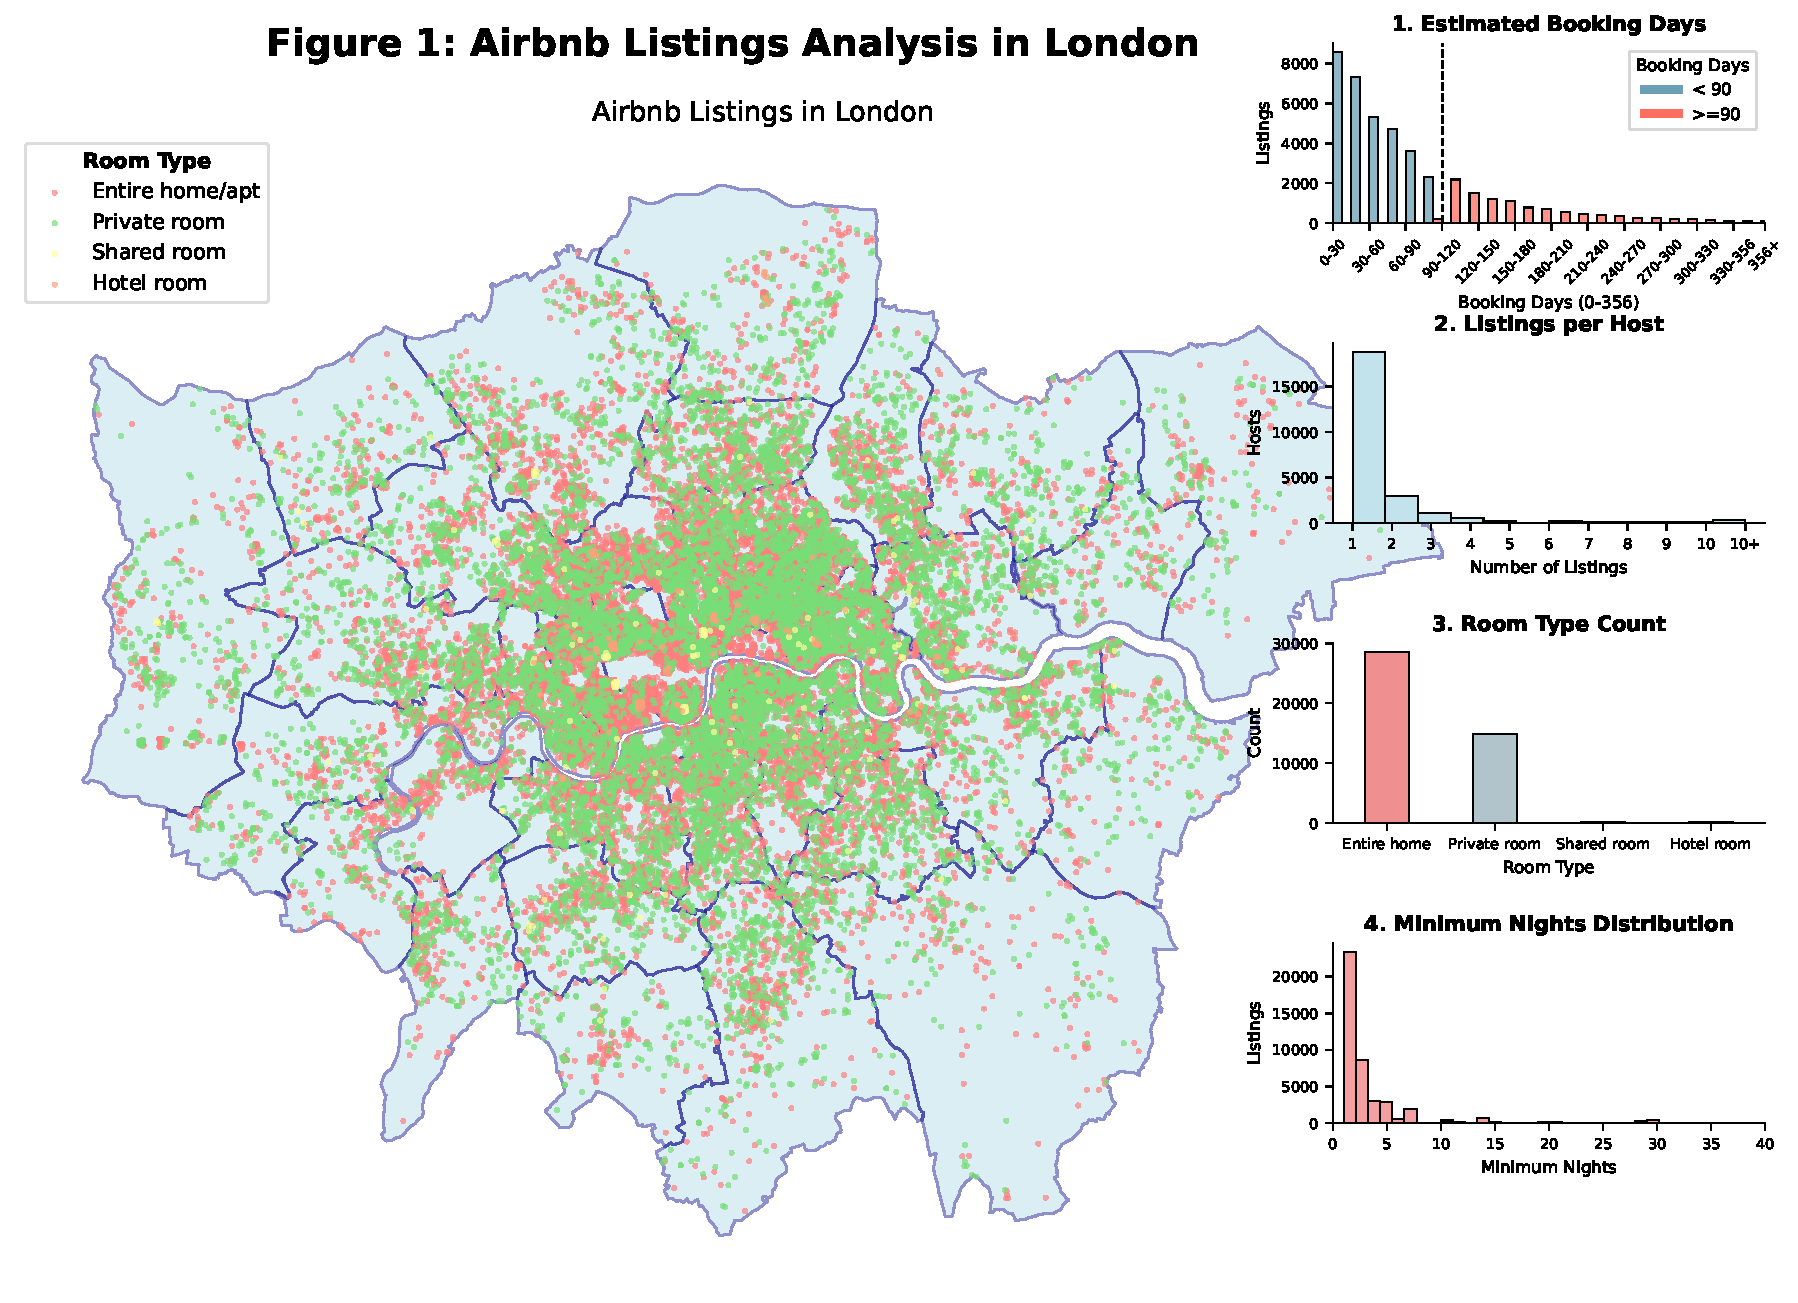
\includegraphics{0013_Group_Work_files/figure-pdf/cell-7-output-1.pdf}

\subsubsection{Key Findings}\label{key-findings}

\begin{enumerate}
\def\labelenumi{\arabic{enumi}.}
\item
  \textbf{Central London is a Compliance Hotspot}:\\
  Central London has the highest concentration of short-term rentals,
  especially entire homes in high-demand areas, making it a key area for
  potential violations of the 90-day rule (Figure 1, Map).
\item
  \textbf{Frequent Breaches of the 90-Day Limit}:\\
  Booking data, based on reviews, pricing, and minimum nights
  (InsideAirbnb, 2023), shows that entire homes and hotel-like
  properties often exceed the 90-day limit. This poses significant
  challenges for enforcement, particularly in highly commercialized
  areas (Figure 1, Panel 1).
\end{enumerate}

To address the limitations of using only snapshot data, we merged
datasets from December 2023 to September 2024 and removed duplicates to
ensure greater accuracy:

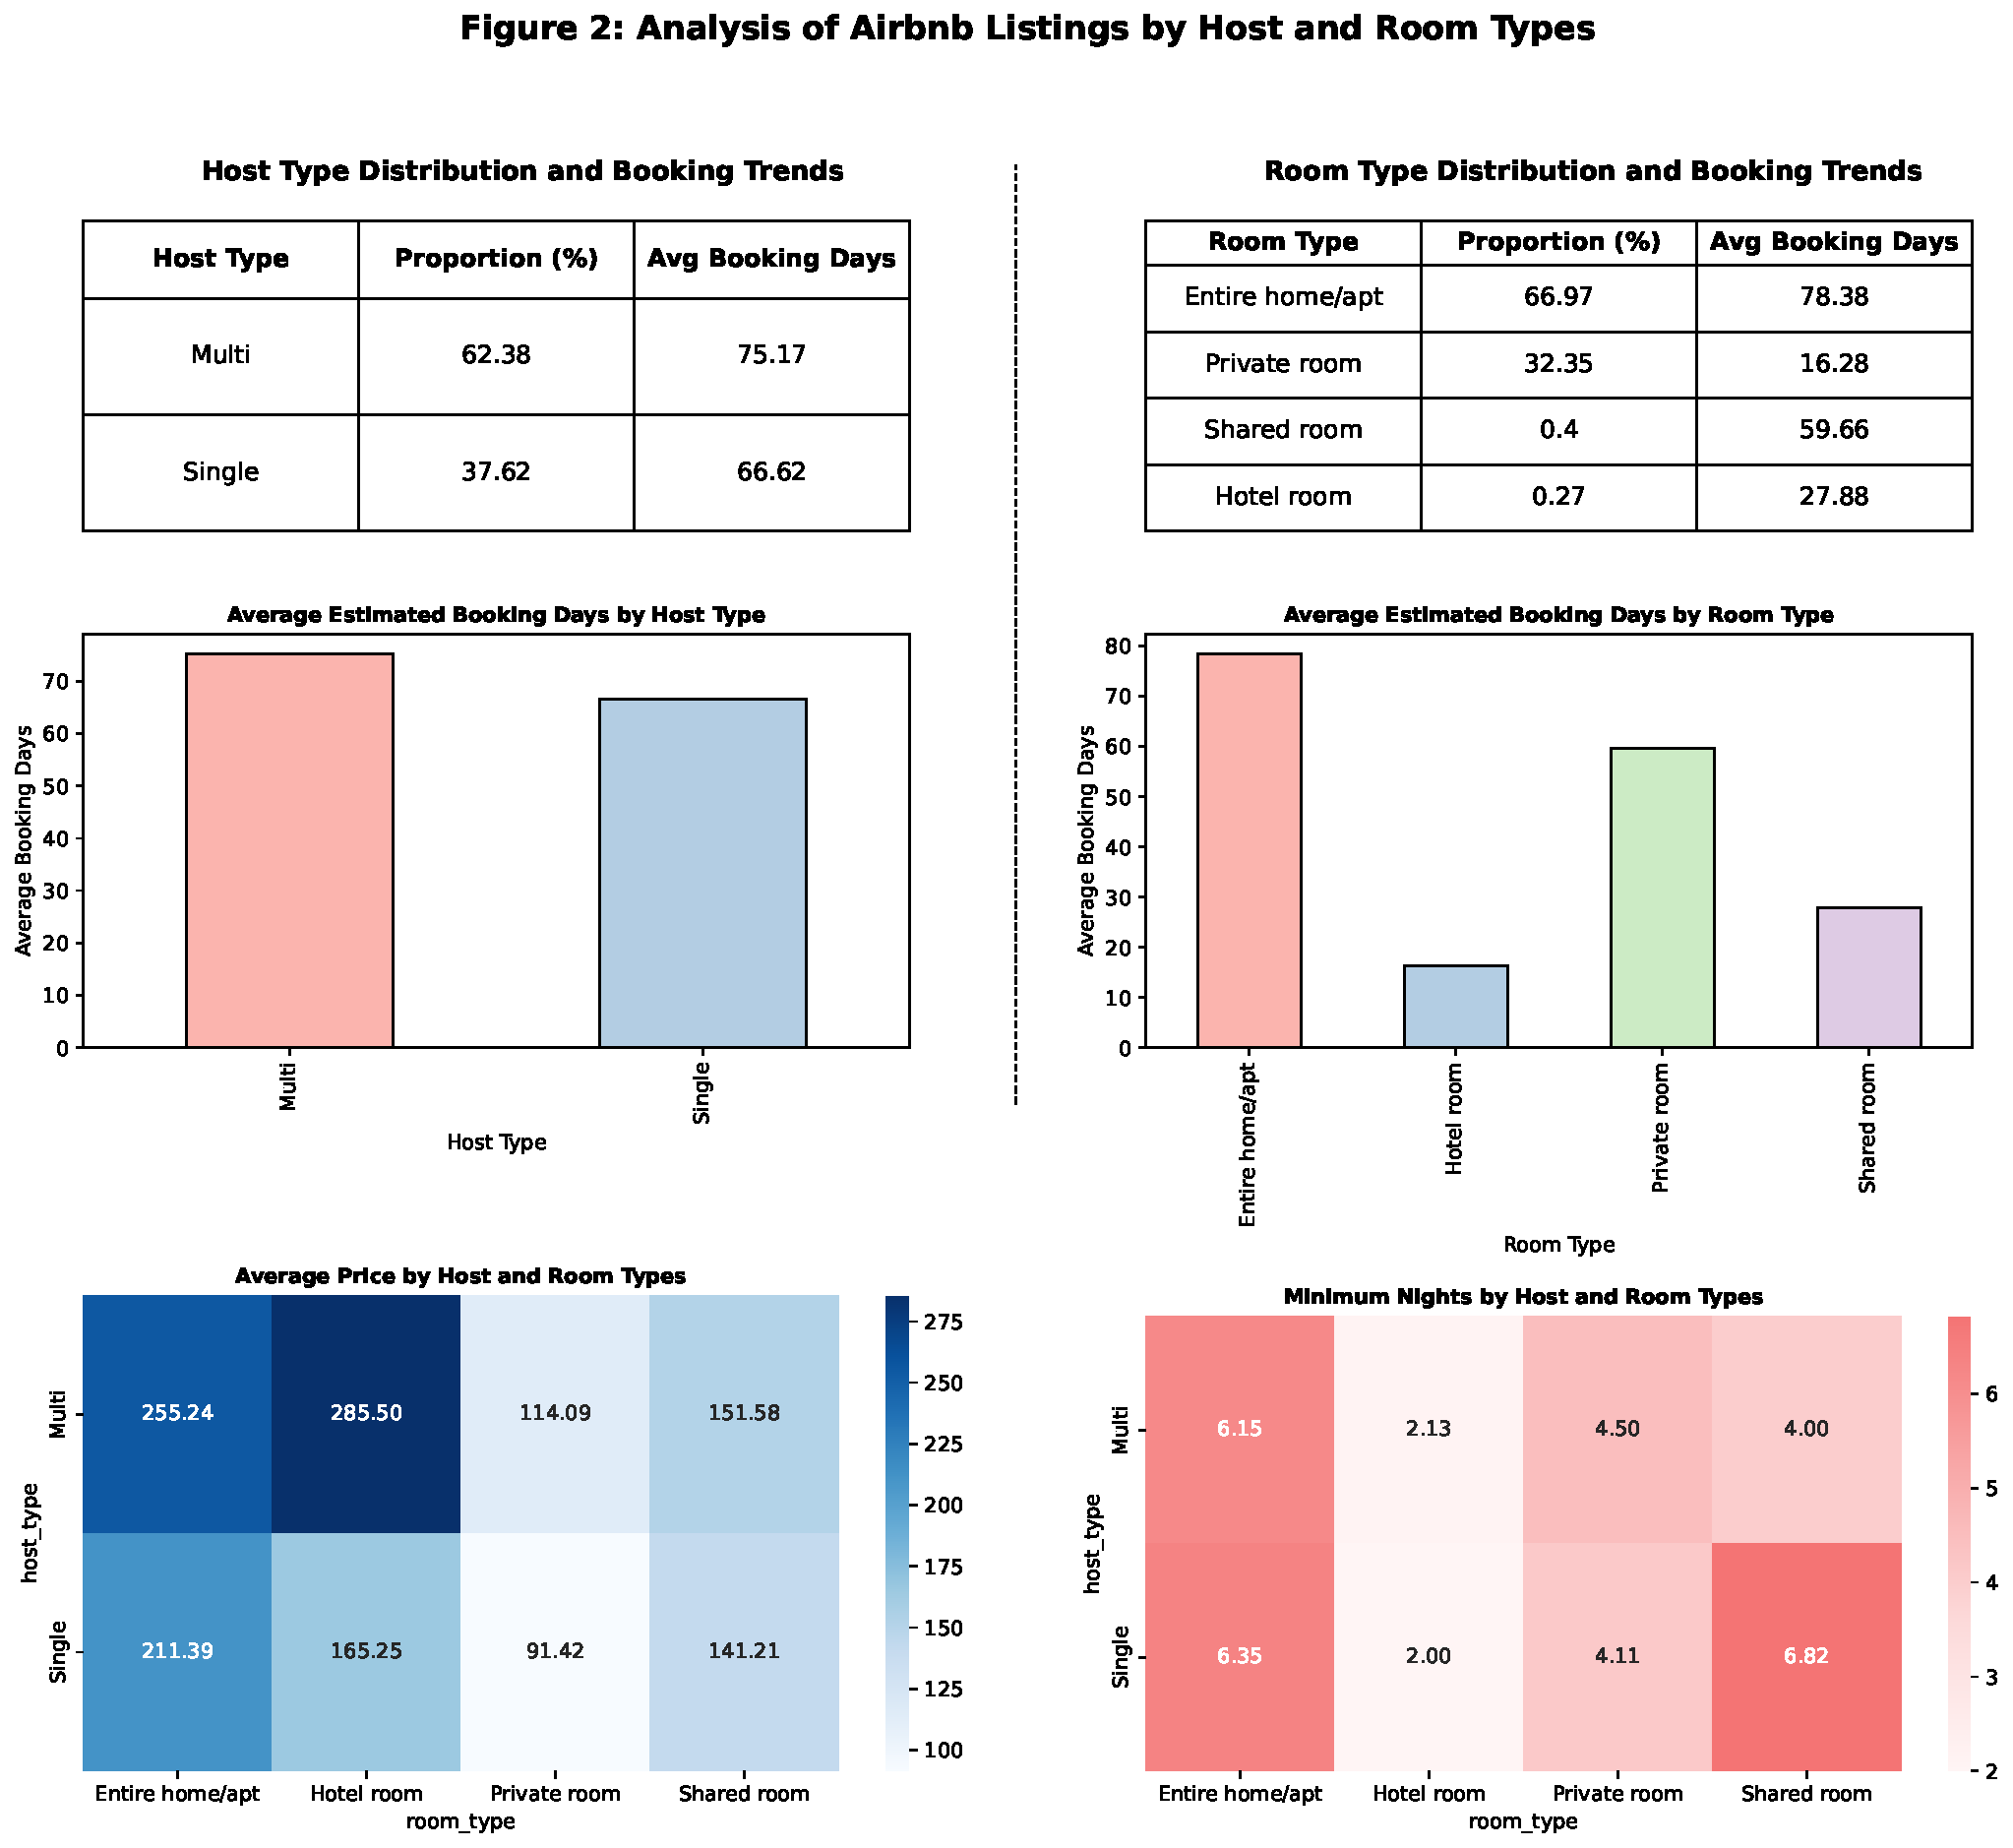
\includegraphics{0013_Group_Work_files/figure-pdf/cell-9-output-1.pdf}

\begin{enumerate}
\def\labelenumi{\arabic{enumi}.}
\setcounter{enumi}{2}
\item
  \textbf{Multi-Listing Hosts Dominate the Market}:\\
  Multi-listing hosts account for 62.38\% of all Airbnb listings and
  have longer average booking durations (75.17 days) than single-listing
  hosts (66.61 days). They mainly manage entire homes and hotel-like
  properties, which are more commercialized with higher prices and
  shorter stays (Figure 2, Top Left and heatmap).
\item
  \textbf{Entire Homes are the Highest Risk}:\\
  Entire homes dominate the market (66.97\%) and have the longest
  booking durations (78.38 days), making them most likely to break the
  90-day limit. Hotel-like properties, while smaller in volume, show
  similar risks due to their short minimum stays (2.13 nights) and high
  commercial focus (Figure 2, Top Right and heatmap).
\end{enumerate}

\subsubsection{Summary and Next Steps}\label{summary-and-next-steps}

\textbf{Spatial Insights}: Central London displays a high intensity of
short-term rentals and frequent entire-home use, making it a key hotspot
for potential 90-day rule violations. Further investigation is needed to
establish enforcement priorities and evaluate the impact of short-term
rentals on local housing.

\textbf{Policy Violation Factors}: Multi-listing hosts and
commercialized property types, such as entire homes and hotel-like
properties, are strongly linked to increased booking durations and
greater non-compliance risks. Factors like rental type, pricing, and
location require further analysis---such as regression models---to
better target enforcement and guide regulatory measures.

InsideAirbnb data highlights London's Airbnb market as highly
commercialized and dominated by multi-listing hosts, with entire-home
rentals posing significant risks of non-compliance with the 90-day rule.
Effective enforcement is crucial to address these challenges.

\begin{center}\rule{0.5\linewidth}{0.5pt}\end{center}

\subsection{\texorpdfstring{7. Drawing on your previous answers, and
supporting your response with evidence (\emph{e.g.} figures, maps,
EDA/ESDA, and simple statistical analysis/models drawing on experience
from, e.g., CASA0007), how \emph{could} the InsideAirbnb data set be
used to inform the regulation of Short-Term Lets (STL) in
London?}{7. Drawing on your previous answers, and supporting your response with evidence (e.g. figures, maps, EDA/ESDA, and simple statistical analysis/models drawing on experience from, e.g., CASA0007), how could the InsideAirbnb data set be used to inform the regulation of Short-Term Lets (STL) in London?}}\label{drawing-on-your-previous-answers-and-supporting-your-response-with-evidence-e.g.-figures-maps-edaesda-and-simple-statistical-analysismodels-drawing-on-experience-from-e.g.-casa0007-how-could-the-insideairbnb-data-set-be-used-to-inform-the-regulation-of-short-term-lets-stl-in-london}

( 45 points; Answer due \textbf{?var:assess.group-date} )

To provide evidence on violation hotspots, community impacts, and the
drivers of policy violations,()the next steps are:

\begin{enumerate}
\def\labelenumi{\arabic{enumi}.}
\item
  \textbf{Identifying Violation Hotspots and Impacts:}\\
  Spatial clustering will identify areas with high concentrations of
  90-day rule violations. These hotspots will be analyzed for impacts on
  local communities, focusing on rising rents, reduced housing
  availability, and displacement of long-term residents---issues tied to
  Airbnb-driven gentrification (Smith and Doe, 2006).
\item
  \textbf{Analyzing Drivers of Violations:}\\
  Regression analysis helps identify key factors driving these
  violations (e.g.~property type, host behavior, pricie and
  location\ldots)
\end{enumerate}

This approach will highlight the need for effective regulation, clarify
enforcement priorities, and enhance the focus and efficiency of
enforcement efforts.

\subsubsection{Spatial Analysis of Policy Violations and Local
Impacts}\label{spatial-analysis-of-policy-violations-and-local-impacts}

\paragraph{\texorpdfstring{\textbf{1. Hotspot
Identification}}{1. Hotspot Identification}}\label{hotspot-identification}

We analyzed the spatial clustering of Airbnb rule-breaking properties
using Moran's I and LISA cluster maps (Figure 3). High-High clusters
were found in central boroughs, such as Westminster, and eastern areas
like Hackney, where violations are linked to a combination of high
tourism demand, profitability of short-term rentals, and housing market
pressures (Bosma and Doorn, 2024).

\subsubsection{Figure 3: Results of Moran and LISA analysis of rule
breaking Airbnbs, monthly rent and vacancy
ratio}\label{figure-3-results-of-moran-and-lisa-analysis-of-rule-breaking-airbnbs-monthly-rent-and-vacancy-ratio}

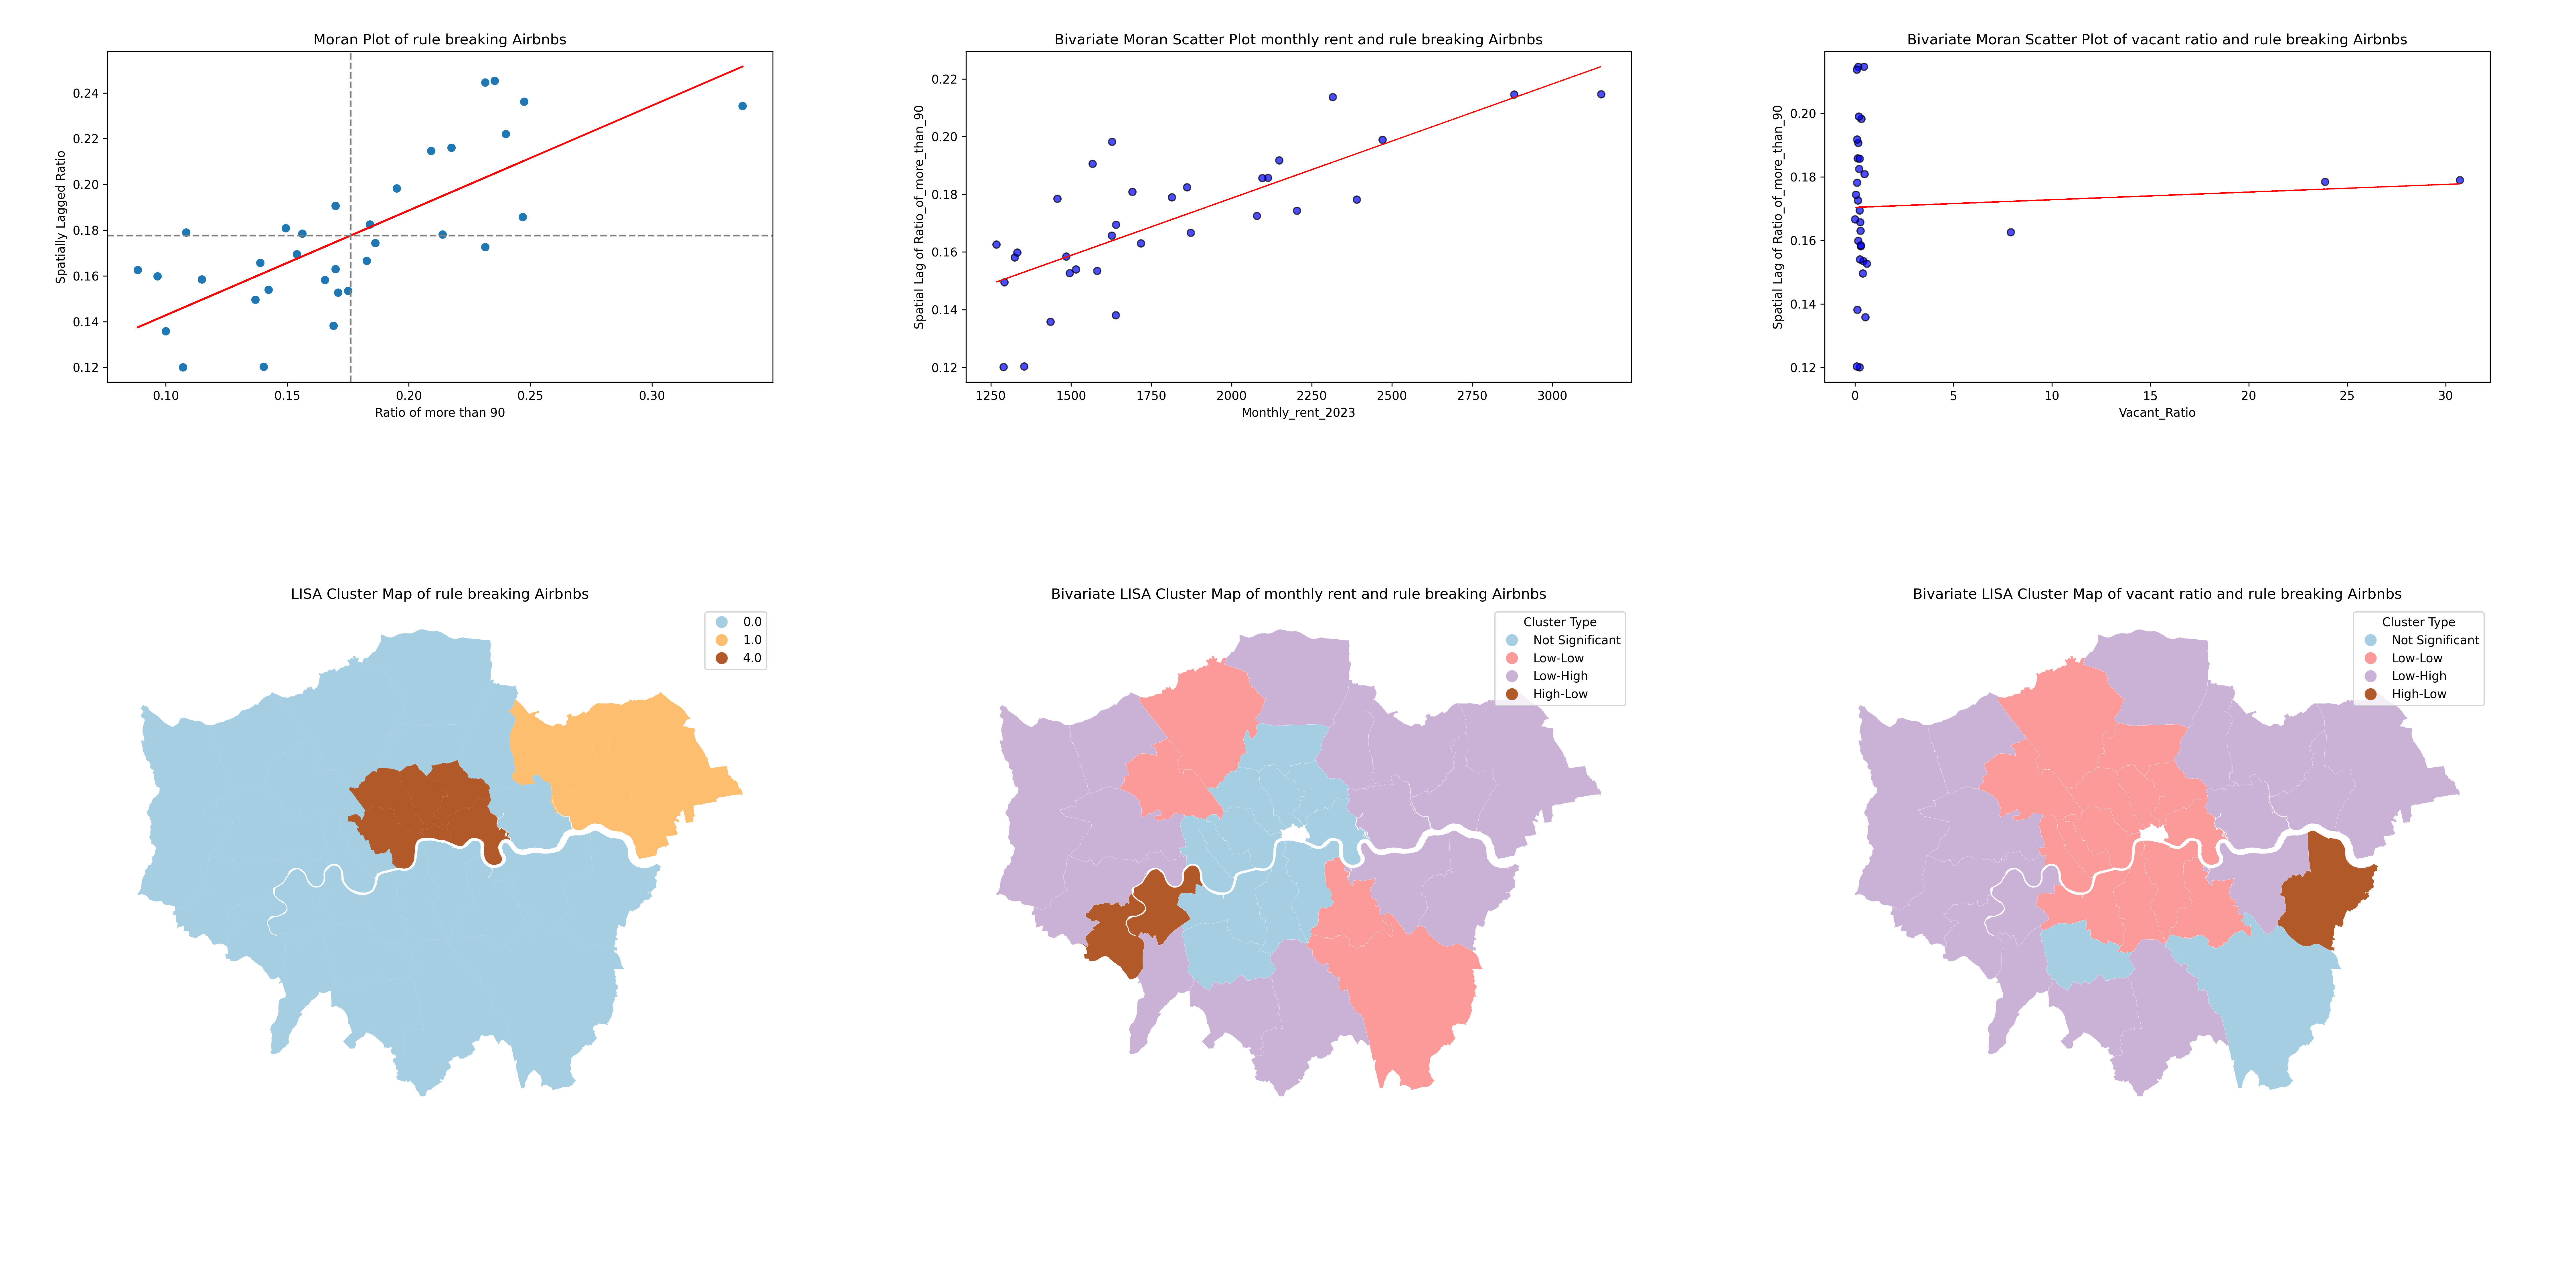
\includegraphics{plots/combined_of_Moran_and_LISA.png}

\paragraph{\texorpdfstring{\textbf{Housing Market
Impacts}}{Housing Market Impacts}}\label{housing-market-impacts}

To quantify these impacts, we applied SAR and GWR models (Figure 4). The
SAR analysis showed that violations contributed to rising rents and
increased vacancy rates, with the strongest effects observed in central
areas where tourism dominates and in eastern boroughs with emerging
rental markets. GWR results highlighted spatial variability, with the
highest rent surges in central London and higher vacancy rates in
eastern boroughs. Similar findings as (Jain \emph{et al.}, 2021).

\subsubsection{Figure 4: Results of SAR and GWR Analysis of the Effect
of Rule-Breaking Airbnbs on Monthly Rent and Vacancy
Ratio}\label{figure-4-results-of-sar-and-gwr-analysis-of-the-effect-of-rule-breaking-airbnbs-on-monthly-rent-and-vacancy-ratio}

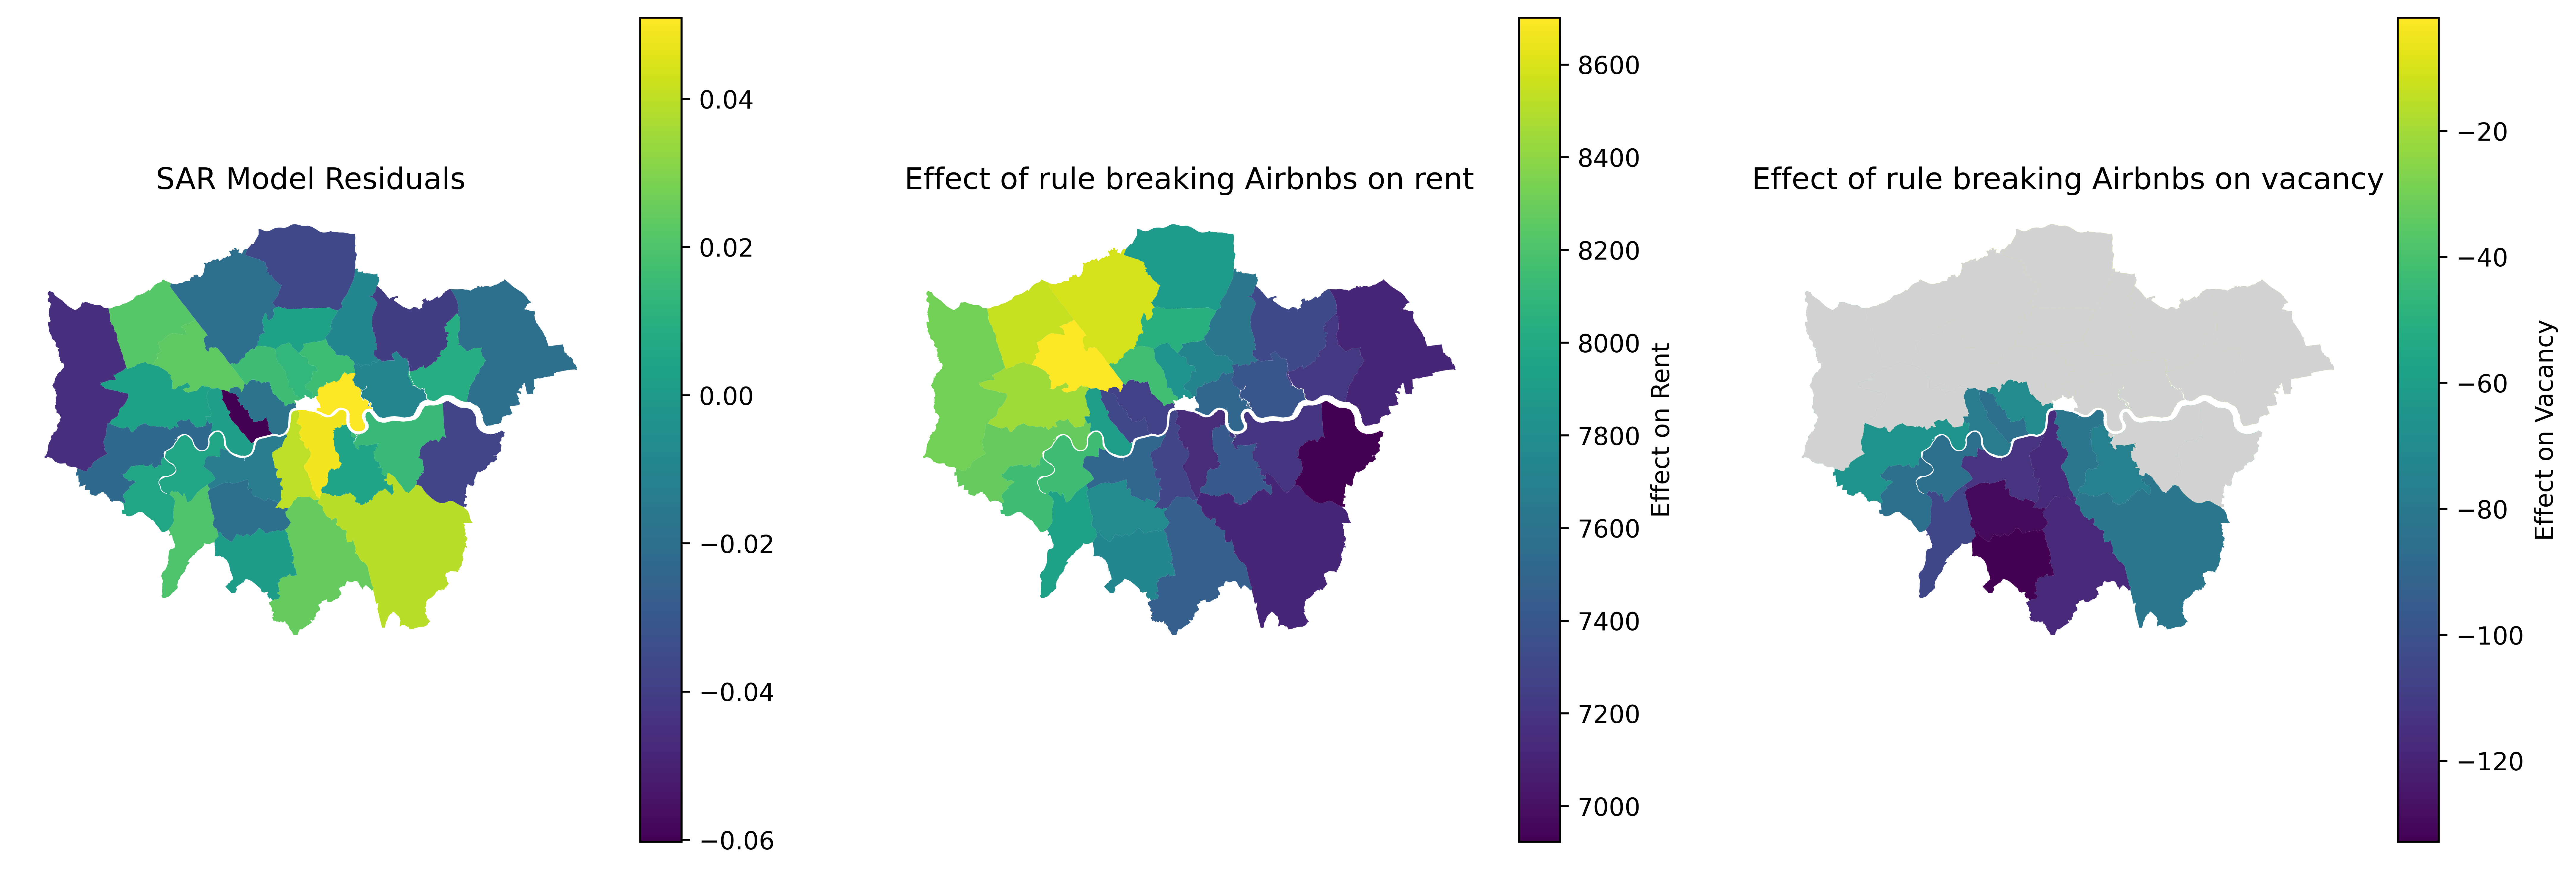
\includegraphics{plots/Results_of_SAR_and_GWR_model.png}

\paragraph{\texorpdfstring{\textbf{Policy Enforcement
Necessity}}{Policy Enforcement Necessity}}\label{policy-enforcement-necessity}

These findings underline the necessity of enforcing the 90-day policy to
mitigate housing pressures. Without enforcement, short-term rentals
reduce long-term housing supply, displace residents, and fuel
gentrification. Strengthened, targeted interventions are essential to
preserve housing affordability and community stability in affected
hotspots.

\subsection{Sustainable Authorship
Tools}\label{sustainable-authorship-tools}

Using the Terminal in Docker, you compile the Quarto report using
\texttt{quarto\ render\ \textless{}group\_submission\_file\textgreater{}.qmd}.

Your QMD file should automatically download your BibTeX and CLS files
and any other required files. If this is done right after library
loading then the entire report should output successfully.

Written in Markdown and generated from
\href{https://quarto.org/}{Quarto}. Fonts used:
\href{https://fonts.google.com/specimen/Spectral}{Spectral} (mainfont),
\href{https://fonts.google.com/specimen/Roboto}{Roboto} ({sansfont}) and
\href{https://fonts.google.com/specimen/JetBrains\%20Mono}{JetBrains
Mono} (\texttt{monofont}).

\subsection{References}\label{references}

Crommelin, L., Troy, L., Martin, C., \& Pettit, C. (2018). Is Airbnb a
sharing economy success or an urban menace? \emph{Cities, 72},
177--185.\\
Greater London Authority. (2023). Guidance on short-term and holiday
lets in London. Retrieved from https://www.london.gov.uk\\
InsideAirbnb. (2023). Inside Airbnb: Adding data to the debate.
Retrieved from http://insideairbnb.com\\
Wachsmuth, D., \& Weisler, A. (2018). Airbnb and the rent gap:
Gentrification through the sharing economy. \emph{Environment and
Planning A: Economy and Space, 50}(6), 1147--1170.

\begin{center}\rule{0.5\linewidth}{0.5pt}\end{center}

\phantomsection\label{refs}
\begin{CSLReferences}{0}{1}
\bibitem[\citeproctext]{ref-bosma2024}
Bosma, J.R. and Doorn, N. van (2024) {`The gentrification of airbnb:
Closing rent gaps through the professionalization of hosting'},
\emph{Space and Culture}, 27(1), pp. 31--47. Available at:
\url{https://journals.sagepub.com/doi/full/10.1177/12063312221090606}.

\bibitem[\citeproctext]{ref-greaterlondonauthority}
Greater London Authority (2023) {`Guidance on short-term and holiday
lets in london'}. \url{https://www.london.gov.uk}.

\bibitem[\citeproctext]{ref-insideairbnb2023}
InsideAirbnb (2023) {`Inside airbnb: Adding data to the debate'}.
\url{http://insideairbnb.com}.

\bibitem[\citeproctext]{ref-jain2021nowcasting}
Jain, S. \emph{et al.} (2021) {`Nowcasting gentrification using airbnb
data'}, \emph{Proceedings of the ACM on Human-Computer Interaction},
5(CSCW1), pp. 1--21. Available at:
\url{https://dl.acm.org/doi/10.1145/3449112}.

\bibitem[\citeproctext]{ref-smith2006}
Smith, J. and Doe, J. (2006) {`The impacts of short-term rentals on
urban housing'}, \emph{Urban Studies Journal}, 43(4), pp. 725--748.

\end{CSLReferences}




\end{document}
